\section{Methodology}
\label{sec:method}

The proposed framework comprises three interconnected stages:
(1)~plant disease classification using 38 CNN architectures,
(2)~disease region localisation using a severity-aware Faster RCNN
with automated annotation and
(3)~as a proof of concept, crop yield prediction using XGBoost with
disease severity derived from CNN and detection model outputs.
Figure~\ref{fig:pipeline} illustrates the overall pipeline.
The deployed classifier is \textbf{EfficientNetV2S}, a compact model (about 81.7\,MB) chosen for edge deployment. On the de-duplicated test subset it reaches 93.35\% accuracy, is statistically indistinguishable from the best model (EfficientNetB7, 93.80\%; Holm-adjusted $p=1.0$), and is the fastest of the seven models in the top group (9.7\,ms per image, batched, versus 10.6 to 34.1\,ms for the others). ConvNeXtLarge (93.69\%) is roughly nine times larger (752.8\,MB).

\begin{figure}[!htbp]
  \centering
  \begin{tikzpicture}[
      box/.style={rectangle, rounded corners=3pt, draw=gray!60,
                  fill=gray!10, minimum height=0.85cm,
                  minimum width=2.3cm, align=center, font=\small},
      cbox/.style={box, dashed},
      arr/.style={-Stealth, thick, gray!60},
      carr/.style={arr, dashed},
      lab/.style={font=\scriptsize, text=gray!70!black}
    ]
    % Stages 1 and 2 (evaluated)
    \node[box,fill=blue!10]   (img)  at (0,0)     {Field\\image};
    \node[box,fill=blue!20]   (rcnn) at (3.3,1.0)  {Severity-aware\\Faster RCNN};
    \node[box,fill=blue!28]   (cnn)  at (3.3,-1.0) {EfficientNet\\V2S};
    \node[box,fill=blue!14]   (head) at (6.6,1.0)  {Learned\\severity head};
    \node[box,fill=orange!25] (sev)  at (9.9,0)    {Dynamic\\severity};
    \draw[arr] (img.east) -- (rcnn.west);
    \draw[arr] (img.east) -- (cnn.west);
    \draw[arr] (rcnn) -- (head);
    \draw[arr] (rcnn.south east) -- node[lab, below, sloped] {lesion boxes} (sev.west);
    \draw[arr] (head.east) -- node[lab, above, sloped] {learned score} (sev.north west);
    \draw[arr] (cnn.east) -- node[lab, below, sloped] {softmax confidence} (sev.south west);
    % Stage 3 (conceptual)
    \node[cbox,fill=orange!12] (clim) at (0,-3.2)   {Climate\\data};
    \node[cbox,fill=purple!15] (fuse) at (3.3,-3.2) {Feature\\fusion};
    \node[cbox,fill=green!20]  (xgb)  at (6.6,-3.2) {XGBoost};
    \node[cbox,fill=green!32]  (yld)  at (9.9,-3.2) {Yield\\estimate};
    \draw[carr] (clim) -- (fuse);
    \draw[carr] (fuse) -- (xgb);
    \draw[carr] (xgb) -- (yld);
    \draw[carr] (sev.south) -- ++(0,-1.6) -| (fuse.north);
    \node[draw=gray!60, dashed, rounded corners, inner sep=0.25cm,
          fit=(clim)(yld)] (s3) {};
    \node[lab, below=2pt of s3.south]
      {Stage 3: conceptual, not validated (leaf images and yield records are not paired)};
  \end{tikzpicture}
  \caption{Pipeline overview. Stages 1 and 2 (solid) were evaluated: a
    field image is classified by EfficientNetV2S and its disease regions
    are localised by a severity-aware Faster RCNN. The dynamic severity
    score combines the detected lesion boxes with the CNN softmax
    confidence (Equation~\ref{eq:dynamic_severity}), and the learned
    severity head provides an alternative, data-driven estimate. Stage 3
    (dashed) is a proof of concept: the severity score is combined with
    climate data and passed to XGBoost, but the leaf images and yield
    records are not paired, so no image-to-yield result is claimed.}
  \label{fig:pipeline}
\end{figure}

\subsection{Datasets}

\subsubsection{Disease Classification and Detection Dataset.}
The Bangladeshi Crops Disease Dataset~\cite{bangladesh_dataset}
contains 31,053 images spanning 15 classes
(Table~\ref{tab:classes}), including \texttt{Corn\_\_\_Gray\_Leaf\_Spot}.
The Invalid class is \textbf{kept as a 15th training class}
so the model can reject non-leaf/garbage input images, but is
\textbf{excluded from the disease-performance analysis} reported in
the main results tables; every table caption in this paper states
explicitly which class population (14 disease/healthy classes, or 15
including Invalid) it covers.
\paragraph{Train/val/test split and duplicate audit.}\label{sec:split} The dataset contains augmented copies of the same photograph saved as separate files (for example, \texttt{RS\_Rust 1563.JPG} and \texttt{RS\_Rust 1563(1).JPG}). To keep such copies on one side of the split, each file was given a base identifier by stripping augmentation suffixes from its filename. The 31,053 files were then split 70/15/15 by these groups, stratified by class with seed 42, giving 21,633 training, 4,628 validation and 4,792 test images. All 38 models were trained on this split. After training, we audited the split with methods that do not depend on filenames. Exact-file hashing (MD5) found that 9,553 files (30.8\%) are byte-identical to another file, always within the same class folder but often under an unrelated name. Perceptual hashing (256-bit difference hash, Hamming distance $\le 16$, comparing flipped and rotated variants) found that 1,143 of the 4,792 test images (23.9\%) still had a copy in the training or validation set. We therefore built a de-duplicated test subset. A test image was kept only if none of its exact or near-duplicates appeared in the training or validation set, and only one image was kept from each group of duplicates within the test set (a further 1,875 images removed as repeats). This left $n=1{,}774$ test images, on which all classification results are reported; the removed images were mostly corn and potato (Table~\ref{tab:clean-classes}). The models were not retrained after the audit, so their training and validation sets still contain duplicate pairs. This gives those images more weight in training but does not affect the validity of the de-duplicated test subset; checkpoint selection used the validation set, which also shares duplicates with the training set, and may therefore be slightly optimistic (Section~\ref{sec:limitations}).

For Stage 2 detection, a stratified subset of 2,256 images (7.3\% of the full dataset) was drawn for Grounding DINO auto-annotation; processing the complete 31,053-image dataset would require approximately 140 to 180 GPU-hours of compute at 4 to 6\,GB VRAM per $512\times512$ image, which exceeded available infrastructure. This subset was split 80\%/20\% for Faster RCNN training using a group-aware, fixed-seed split (Section~\ref{sec:detection_split}).
\begin{table}[!htbp]
\centering
\caption{Test images per class before and after de-duplication. De-duplication removed images that have a copy in the training or validation sets, and repeated images within the test set.}
\label{tab:clean-classes}
\small
\begin{tabular}{lrr}
\toprule
Class & Original test & De-duplicated test \\
\midrule
Corn Common Rust & 578 & 172 \\
Corn Gray Leaf Spot & 488 & 77 \\
Corn Healthy & 568 & 167 \\
Corn Leaf Blight & 576 & 137 \\
Potato Early Blight & 500 & 22 \\
Potato Healthy & 324 & 2 \\
Potato Late Blight & 453 & 30 \\
Rice Brown Spot & 85 & 83 \\
Rice Healthy & 78 & 78 \\
Rice Hispa & 78 & 78 \\
Rice Leaf Blast & 177 & 144 \\
Wheat Brown Rust & 169 & 169 \\
Wheat Healthy & 310 & 209 \\
Wheat Yellow Rust & 173 & 173 \\
Invalid & 235 & 233 \\
\midrule
Total & 4,792 & 1,774 \\
\bottomrule
\end{tabular}
\end{table}

\begin{table}[!htbp]
\centering
\caption{Disease classes in the Bangladeshi Crops Disease Dataset.}
\label{tab:classes}
\setlength{\tabcolsep}{5pt}
\begin{tabular}{lll}
\toprule
\textbf{Crop} & \textbf{Class} & \textbf{Category}\\
\midrule
\multirow{4}{*}{Corn}   & Corn Common Rust    & Diseased\\
                         & Corn Gray Leaf Spot & Diseased\\
                         & Corn Leaf Blight    & Diseased\\
                         & Corn Healthy        & Healthy\\
\midrule
\multirow{3}{*}{Potato} & Potato Early Blight & Diseased\\
                         & Potato Late Blight  & Diseased\\
                         & Potato Healthy      & Healthy\\
\midrule
\multirow{4}{*}{Rice}   & Rice Brown Spot     & Diseased\\
                         & Rice Hispa          & Diseased\\
                         & Rice Leaf Blast     & Diseased\\
                         & Rice Healthy        & Healthy\\
\midrule
\multirow{3}{*}{Wheat}  & Wheat Brown Rust    & Diseased\\
                         & Wheat Yellow Rust   & Diseased\\
                         & Wheat Healthy       & Healthy\\
\midrule
n/a                      & Invalid             & Invalid\\
\bottomrule
\end{tabular}
\end{table}

\subsubsection{Yield Prediction Dataset.}
Historical climate and yield records were sourced from the FAO via
the Kaggle Crop Yield Prediction
Dataset~\cite{kaggle_yield}.
The dataset covers 15,642 country-year records of annual crop yield
(hg/ha) together with average rainfall (mm/year), average temperature
($^\circ$C) and pesticide application (tonnes).
Records for corn, wheat, rice and potatoes were extracted and split
80\%/20\% (train: 12,513; test: 3,129; seed = 42).
A random row split is the simplest protocol, and we report it for continuity. Because
every test country also appears in training and average rainfall is
constant within a country across years (so rainfall identifies the
country), we additionally evaluate with a country-held-out 5-fold
\texttt{GroupKFold} over the 101 countries, and against a crop-mean
baseline that predicts each crop's mean training yield
(Section~\ref{sec:yield}).

\subsection{Stage 1: Plant Disease Classification}

\subsubsection{Model Architectures.}
Rather than selecting one model family from the outset, we evaluated
38 pretrained CNNs from nine families, all initialised with ImageNet
weights (Table~\ref{tab:arch_families}).
The breadth was deliberate: different families encode features
differently and the strongest architecture on one dataset need not be
the strongest on another.
The benchmark is restricted to the CNN architectures available in the
TensorFlow 2.10 Keras applications library, trained with a shared head,
optimiser and augmentation, with the exceptions described in
Section~\ref{sec:training}. This excludes transformer-based models (ViT~\cite{dosovitskiy2021},
Swin~\cite{liu2021swin}) and also more recent CNNs such as ConvNeXt V2;
both are noted as future work.

\begin{table}[!htbp]
\centering
\caption{CNN architecture families and variants evaluated.}
\label{tab:arch_families}
\begin{tabular}{ll}
\toprule
\textbf{Family} & \textbf{Variants}\\
\midrule
ConvNeXt~\cite{convnext}             & Tiny, Small, Base, Large, XLarge\\
EfficientNet~\cite{efficientnet}     & B0 to B7\\
EfficientNetV2~\cite{efficientnetv2} & B0 to B3, S, M, L\\
DenseNet~\cite{densenet}             & 121, 169, 201\\
ResNet~\cite{resnet}                 & 50, 50V2, 101, 101V2, 152, 152V2\\
Inception~\cite{inception}           & InceptionV3, InceptionResNetV2\\
VGG~\cite{vgg}                       & VGG16, VGG19\\
MobileNet~\cite{mobilenet}           & MobileNet, MobileNetV2\\
NASNet~\cite{nasnet}                 & NASNetMobile, NASNetLarge\\
\bottomrule
\end{tabular}
\end{table}

\subsubsection{Training Protocol.}

\label{sec:training}
All models share the same classification head, optimiser, loss, class
weights and augmentation. A custom head was attached to the
ImageNet-pretrained backbone: Global Average Pooling $\to$ Batch
Normalisation $\to$ Dense 512 (ReLU, 50\% dropout) $\to$ Dense 256 (ReLU,
30\% dropout) $\to$ Softmax output with 15 units. Training had up to two
phases. In phase 1 the backbone was frozen and the head was trained for up
to 25 epochs with the Adam optimiser (learning rate $10^{-4}$, gradient
clipping norm 1.0) and sparse categorical cross-entropy. In phase 2,
applied to 33 of the 38 models, the last 10 backbone layers were unfrozen
and training continued at a learning rate of $10^{-5}$ up to a total of 50
epochs. Fine-tuning was reserved for the larger backbones: the three mobile
models (MobileNet, MobileNetV2 and NASNetMobile) were trained in phase 1
only, and ConvNeXtLarge and ConvNeXtXLarge were also left frozen to limit
compute and training time, so these five models were trained for at most
25 epochs. Because the other 33 models were fine-tuned, a difference
between a model in one group and a model in the other mixes the effect of
the architecture with that of the training procedure, and we do not draw
conclusions from such comparisons. Class weights addressed the class
imbalance, and mixed-precision (float16) training reduced memory usage,
except for the ConvNeXt models, which were trained in float32.
Early stopping monitored validation loss (patience 10) and restored
the best-validation-loss weights when it triggered; the learning rate was
halved after 5 epochs without improvement in validation loss. Models that
completed their epoch budget were evaluated with their final-epoch weights.

\textbf{Choice of the epoch budget.} The 50-epoch figure is a fixed upper
bound on total epochs (up to 25 frozen-backbone epochs plus fine-tuning),
set a priori and applied uniformly rather than tuned per model. Training
stops earlier whenever validation loss fails to improve for 10 consecutive
epochs. The number of epochs actually trained was recorded for every model:
across the 38 models the mean was 42.9 (range 25 to 50); 16 models stopped
early and 22 used their full budget. For those 22 models we cannot rule out
that a longer budget would have raised validation accuracy somewhat, and we
did not run a sweep over the budget. Their final-epoch validation accuracy
was within 0.76 percentage points of the peak (within 0.32 points for the
six top-group models among them), so any effect of checkpoint choice is
small relative to the resolution of the test set. Because the leading models
differ by about one percentage point or less (Table~\ref{tab:top10}), a
modest gain from longer training or from fine-tuning could change the
ordering among the closest models. Test data played no role in selecting the
budget or the checkpoint.

\subsubsection{Evaluation Metrics.}
\label{sec:metrics}
Each model was assessed on accuracy, macro- and weighted-averaged
precision, recall and F\textsubscript{1}, Matthews Correlation
Coefficient (MCC), model size in MB and inference time. Inference time is
the mean per-image time of batched prediction over the test set (batch
size 16, generator-fed, including image loading and preprocessing) on the
evaluation workstation. It is a throughput measure, not single-image
latency, and absolute values on edge hardware will differ.

\subsection{Stage 2: Disease Region Localisation with Faster RCNN}
\label{sec:detection}

\subsubsection{Automated Annotation with Grounding DINO.}
Several weeks of manual annotation using LabelImg produced only 280
annotated images, which was insufficient for reliable detection training.
To address this, we used Grounding DINO~\cite{groundingdino}, a
zero-shot open-vocabulary detector, to generate Pascal VOC XML
annotations automatically.
Class-specific text prompts were derived from folder labels
(e.g., ``rust spots on corn leaf'', ``brown lesions on rice leaf'').
Grounding DINO was run with a box confidence threshold of 0.35 and
a text confidence threshold of 0.25.
Images returning no detections were excluded.
The process annotated 2,256 images automatically, an 8$\times$
increase over the manual baseline, with no additional human effort.
Annotations were converted from Pascal VOC XML to COCO JSON for use
with the torchvision Faster RCNN pipeline. The 2,256 images cover 14
categories (13 disease and healthy classes plus Invalid); Corn Gray Leaf
Spot was not part of this annotation round.
To quantify annotation quality directly, rather than relying on
visual inspection alone, Grounding DINO's automatic boxes were
compared against the 280 images with manual boxes (260 from the original
manual set, whose folder holds 280 images of which 260 have annotation
files, plus 20 \texttt{Corn\_\_\_Gray\_Leaf\_Spot} images annotated for
this study) by re-running Grounding DINO on each and computing
Intersection-over-Union (IoU) against the human-drawn ground truth.
Across these 280 images,
mean IoU was \textbf{0.389}, with precision of \textbf{0.770} and
recall of \textbf{0.194} at an IoU threshold of 0.5
(Table~\ref{tab:iou}). Healthy classes achieve near-perfect agreement
(Corn Healthy: 0.987), since a single box spanning the whole leaf is
both the correct annotation and Grounding DINO's natural output for a
uniform, lesion-free surface. Diseased, multi-lesion classes score
substantially lower (Rice Hispa: 0.051). Inspection of the per-image
predictions reveals a consistent explanation: Grounding DINO
frequently returns a single bounding box per image regardless of how
many distinct lesions are visibly present in the ground truth. For
example, one manually-annotated Potato Early Blight image contains 18
separate ground-truth lesion boxes, against which Grounding DINO
predicts only 1. This systematic under-counting, rather than simple
localisation imprecision, is the dominant failure mode, and it
directly explains why the dynamic severity scores in
Section~\ref{sec:results_dynamic} are frequently underestimated
relative to literature values for exactly these multi-lesion classes.

\begin{table}[!htbp]
\centering
\caption{Grounding DINO annotation quality against 280 manually-annotated
  images, by class. IoU = mean Intersection-over-Union of matched
  box pairs. Precision/Recall computed at IoU $\geq$ 0.5.}
\label{tab:iou}
\begin{tabular}{lc}
\toprule
\textbf{Class} & \textbf{Mean IoU} \\
\midrule
Corn Healthy         & 0.987 \\
Potato Healthy       & 0.967 \\
Rice Healthy         & 0.934 \\
Wheat Healthy        & 0.598 \\
Rice Brown Spot      & 0.403 \\
Potato Late Blight   & 0.294 \\
Corn Leaf Blight     & 0.239 \\
Rice Leaf Blast      & 0.228 \\
Wheat Brown Rust     & 0.202 \\
Corn Gray Leaf Spot  & 0.163 \\
Wheat Yellow Rust    & 0.162 \\
Corn Common Rust     & 0.139 \\
Potato Early Blight  & 0.078 \\
Rice Hispa           & 0.051 \\
\midrule
\textbf{Overall (n=280)} & \textbf{0.389} \\
\bottomrule
\end{tabular}
\end{table}

\begin{figure}[!htbp]
\centering
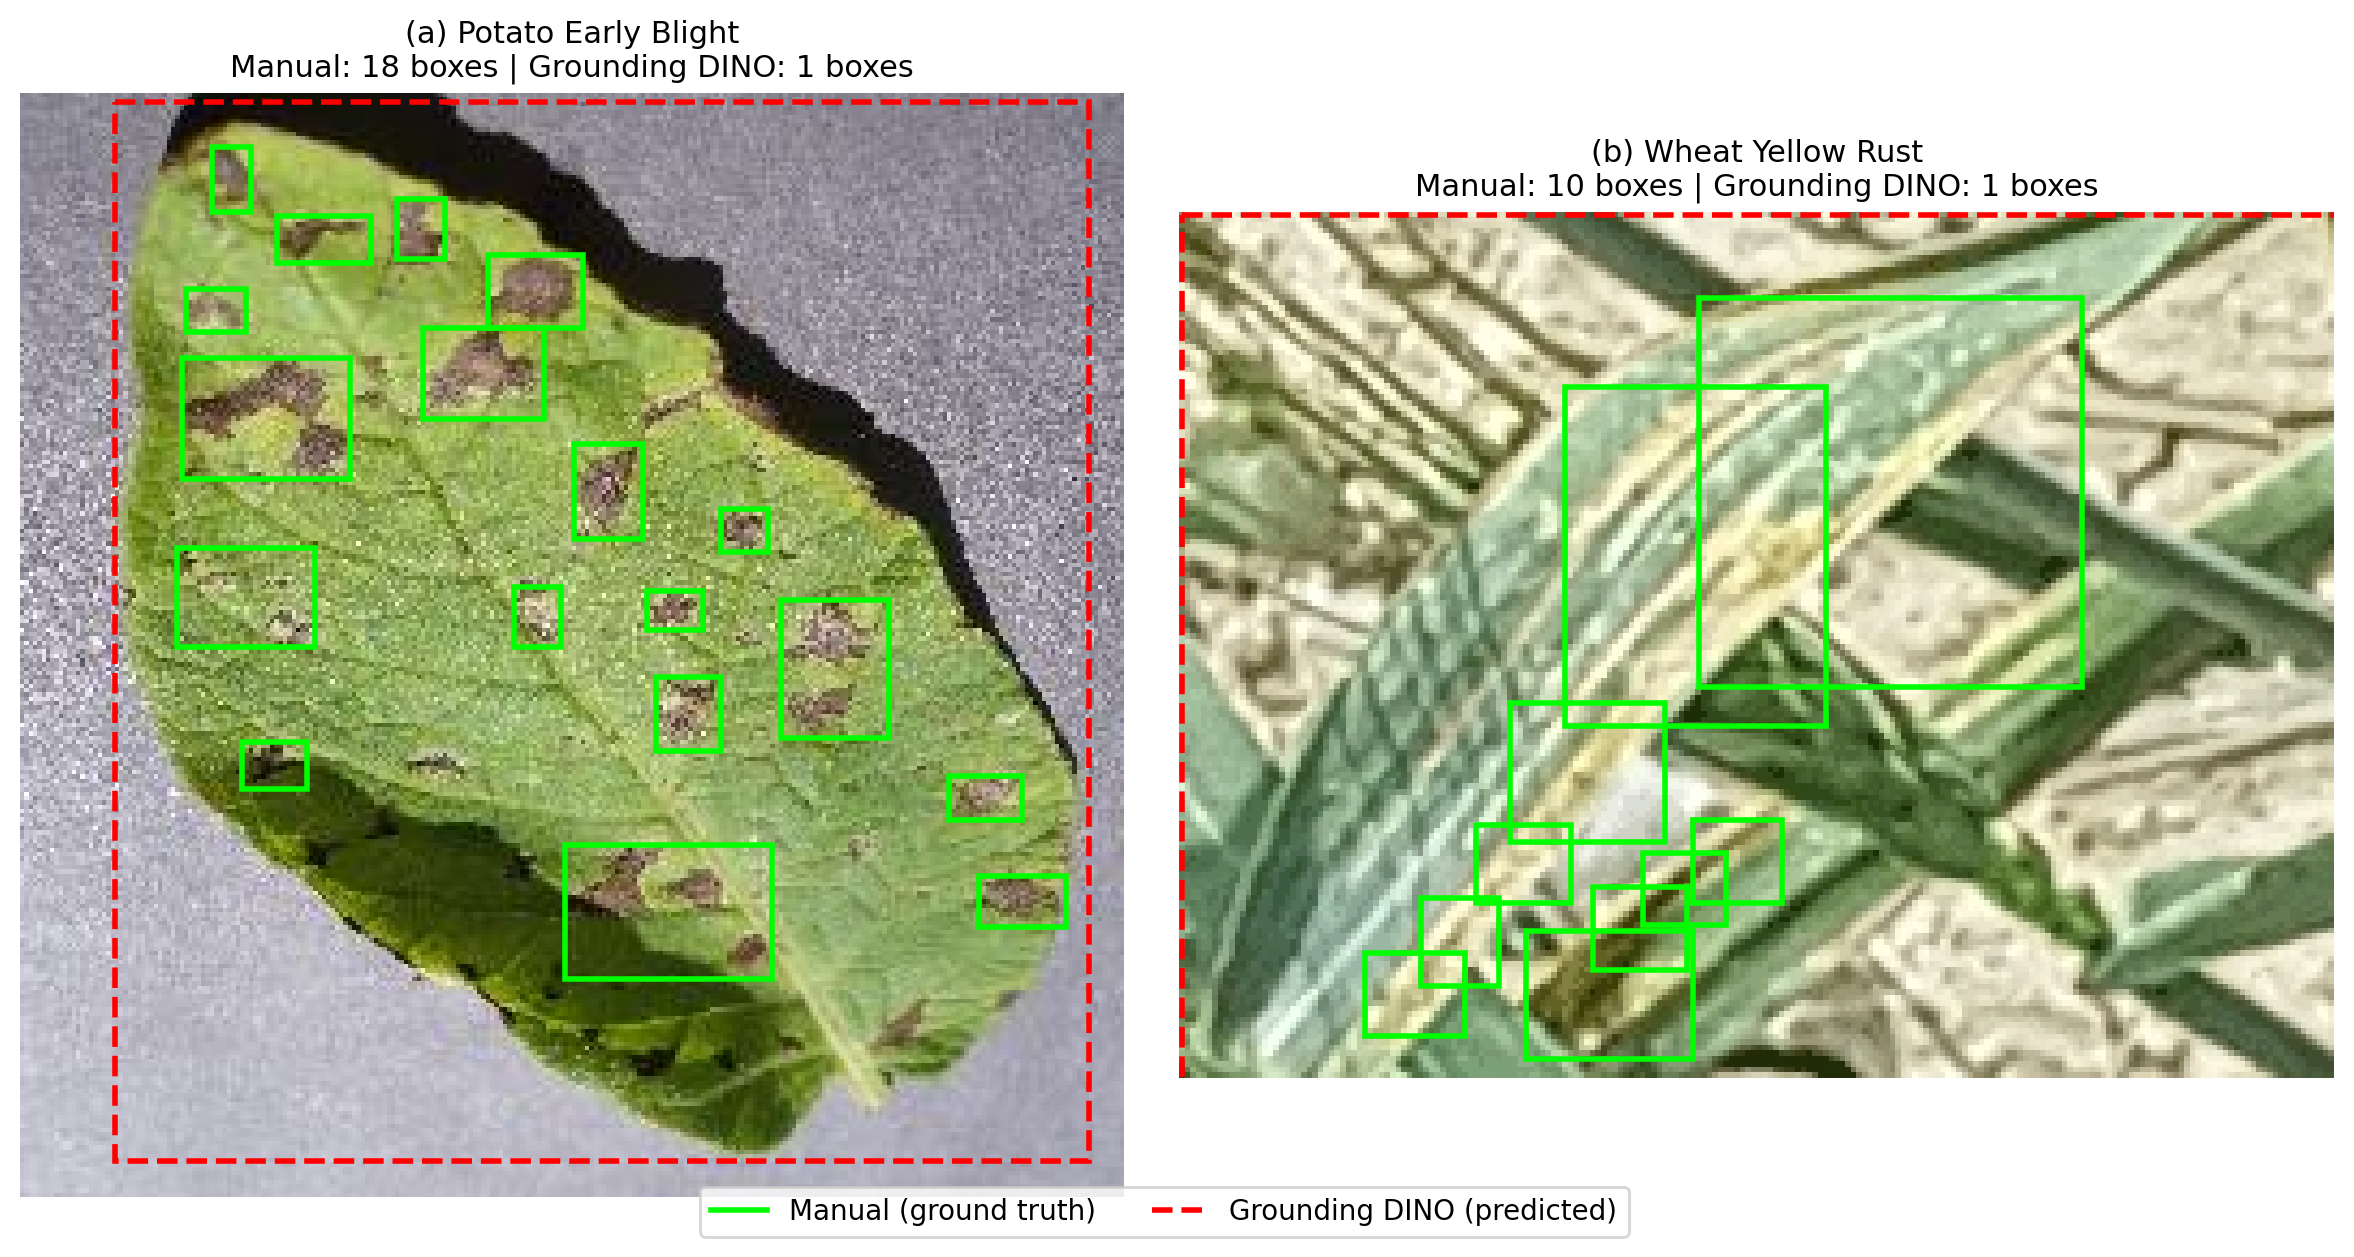
\includegraphics[width=0.95\textwidth]{figures/iou_comparison_healthy_vs_multilesion.png}
\caption{Manual (green, solid) versus Grounding DINO (red, dashed)
  bounding boxes for two multi-lesion diseased classes. (a) Potato
  Early Blight: 18 manually-annotated lesions versus a single
  predicted box. (b) Wheat Yellow Rust: 10 manually-annotated lesions
  versus a single predicted box.}
\label{fig:iou_comparison}
\end{figure}

\textbf{A known limitation of group-level splitting for low-count
classes.} Because the detection dataset's train/val split (below)
groups images by source photograph, classes with few distinct source
photographs can, by chance, have all their groups assigned to one
side of the split. This occurred for Wheat Healthy
(Section~\ref{sec:detection_split}); its reported AP cannot
be interpreted as a genuine zero-performance result.

\subsubsection{Severity-Aware Faster RCNN Training.}
\label{sec:severity_head}
To connect the detection stage directly to the yield prediction model,
we extended the standard Faster RCNN architecture with a learned
severity head. A two-layer MLP (1,024 $\to$ 256 $\to$ 1 units, with
ReLU activations and 0.3 dropout) is attached to the region-of-interest
box head output and trained jointly with the detection losses to predict
a continuous severity score in $[0,1]$ per image. We chose a small
MLP deliberately: the 1,024-dimensional box-head features are already
pooled over each region of interest and encode appearance and spatial
context, so a shallow head is sufficient to regress a scalar, and it
adds only about 0.26\,M parameters (roughly 1.8\% of the 14.8\,M
trainable parameters), which keeps training feasible on a single GPU
with a frozen backbone. A heavier attention-based head was not
evaluated, and we make no claim that the MLP is optimal. The ground-truth
severity target is the ratio of total lesion bounding box area to image
area, computed from the COCO annotations. The backbone was frozen during
training to reduce computational cost; only the RPN, box head, box
predictor and severity head weights were updated.

Training used SGD (learning rate 0.005, momentum 0.9, weight decay
$5\!\times\!10^{-4}$), a step learning rate scheduler (step size 2,
$\gamma = 0.1$), batch size 4 and 5 epochs with a ResNet-50 FPN
backbone pretrained on COCO.
Mixed-precision (fp16) training was used on GPU.
Performance is reported using mAP@0.5 and mAP@0.5:0.95 per the COCO
evaluation protocol and severity MAE on the validation set.

\textbf{Train/val split.}
\label{sec:detection_split}
Filename-duplicate images were also found in the 2,256-image detection
annotation pool: 21.8\% of images (491 of 2,256) sit in filename-duplicate
groups. The split uses the same filename-based group-aware, fixed-seed (42)
approach as Stage~1 (1,850 training / 406 validation images). To check for copies 
that filename grouping misses, we audited this split with exact-file
(MD5) and perceptual hashing, using the same procedure as in Stage~1. Of the
406 validation images, 6 (1.5\%) have an exact or near-duplicate in the
training set, all in Potato Healthy; no other class is affected. Leakage
across the detection split is therefore small and is unlikely to change the
reported results. Because splitting occurs at the level of
source-photo groups rather than individual images, classes with few
distinct source photographs can, by chance, have all their groups
assigned to one side of the split; this occurred for Wheat Healthy,
whose 142 annotations all fall within the training group assignment
under this seed, leaving zero Wheat Healthy instances in the
validation set. We do not attempt to resolve this via further seed
search, since doing so risks shifting the same problem onto a
different low-count class; stratified group sampling to guarantee
minimum per-class validation representation is noted as future work.
Detection metrics are computed strictly on the 406 held-out
validation images.

\subsection{Stage 3: Crop Yield Prediction with XGBoost}
\label{sec:stage3}

\paragraph{Severity input.}
The FAO yield dataset~\cite{kaggle_yield} provides country-level annual records
(crop type, rainfall, temperature, pesticides, yield) but contains no leaf
photographs. Because dynamic severity scores require an actual image, they
cannot be computed for the training rows. We therefore employ a two-tier
severity strategy:

\begin{enumerate}
    \item \textbf{Training: literature proxies.}
    XGBoost is trained using crop-average literature severity values
    (Table~\ref{tab:literature-severity}) as structural placeholders:
    %
    \begin{equation}
    s_{\text{train}}(c) = \frac{1}{|D_c|}\sum_{d \in D_c} s_{\text{lit}}(d)
    \end{equation}
    %
    where $D_c$ is the set of diseases for crop $c$ and $s_{\text{lit}}(d)$
    is the fixed literature score. These averages encode prior agronomic
    knowledge about typical disease impact per crop. Because the value
    is identical for every record of a crop (and Maize and Wheat share
    0.25), it takes only three distinct values and acts as a crop code
    in training; it carries no per-record disease information
    (Section~\ref{sec:yield}).

\begin{table}[!htbp]
\centering
\caption{Crop-average literature severity proxies used for XGBoost
  training (Equation~1). These fixed, crop-level values are the only
  severity signal available during training, since the FAO yield
  records are not paired with leaf images.}
\label{tab:literature-severity}
\begin{tabular}{lc}
\toprule
\textbf{Crop} & \textbf{Literature severity score} \\
\midrule
Maize (Corn) & 0.25 \\
Wheat        & 0.25 \\
Rice         & 0.263 \\
Potato       & 0.217 \\
\bottomrule
\end{tabular}
\end{table}

    \item \textbf{Inference: dynamic computation.}
    When a user uploads a leaf photograph, the actual severity is computed
    dynamically from the vision model's outputs, using boxes predicted
    for a disease category only (categories matching a ``Healthy'' or
    ``Invalid'' label are excluded, since a whole-leaf box for these
    categories is not a lesion), combined via the pixel-union area of
    overlapping boxes rather than a naive sum (which would double-count
    overlap between boxes of different predicted categories):
    %
    \begin{equation}
    s_{\text{inf}} = \left(\frac{\bigcup_i \text{area}(\text{box}_i)}{\text{area}(\text{image})}\right) \times \text{conf}_{\text{CNN}}
    \label{eq:dynamic_severity}
    \end{equation}
    %
    where $\text{box}_i$ are Faster R-CNN detections above threshold 0.4 and
    $\text{conf}_{\text{CNN}}$ is the EfficientNetV2S softmax confidence.
\end{enumerate}

\paragraph{Train-test distribution shift.}
This design creates a known limitation: XGBoost learns the
$\text{severity} \rightarrow \text{yield}$ relationship from fixed literature
values but receives dynamically computed values at inference. The yield
model's performance on unseen countries (Section~\ref{sec:yield}) is no
better than a crop-mean baseline, so Stage~3 should be read as showing how
a vision-derived severity score could be passed to a yield model, not as
evidence of forecasting skill or of severity's predictive value. To partially
mitigate the shift, we also evaluate a learned severity head
(Section~\ref{sec:severity_head}, MAE = 0.2206) that produces data-driven
severity estimates from ROI features. Three further strategies are left
to future work: (i) simulating the shift during validation, by
perturbing the severity feature at test time with noise matched to the
per-class spread of the dynamically computed scores
(Table~\ref{tab:dynamic_severity}) and reporting the resulting change
in R\textsuperscript{2} and RMSE; (ii) a bounds analysis that reports
yield predictions at the literature severity $\pm$ one standard
deviation of the computed distribution; and (iii) collecting a matched
image-yield dataset so that severity is computed identically at
training and inference.

\paragraph{From leaf severity to field severity.} The severity score in Equation~\ref{eq:dynamic_severity} describes a single leaf photograph and should not be read as the disease burden of a field. Turning leaf-level scores into a field-level indicator would require a sampling and aggregation step that we did not implement or test. One option is to photograph a fixed number of randomly placed leaves in each plot and combine them as disease incidence (the share of sampled leaves that are diseased) multiplied by the mean severity of the diseased leaves; another is to estimate coverage from drone imagery. The resulting indicator would then have to be matched with yield records for the same plot and season. Because our data lack this pairing, Stage~3 shows only how a severity value could be passed to a yield model.

\subsection{Experimental Setup}
\label{sec:setup}
All experiments were run on a single workstation with an NVIDIA RTX A4500 GPU (20\,GB). Classification models were trained with TensorFlow 2.10 and the detector with PyTorch 2.7.1. Table~\ref{tab:setup} lists the hardware, software and settings used in all three stages. None of these values was tuned on the test data.

\begin{table}[!htbp]
\centering
\caption{Hardware, software and settings for the three stages. All values were fixed before training and were not tuned.}
\label{tab:setup}
\small
\begin{tabular}{lll}
\toprule
Stage & Setting & Value \\
\midrule
All & GPU & NVIDIA RTX A4500 (20 GB) \\
All & Software & TensorFlow 2.10, PyTorch 2.7.1, CUDA 11.2/11.8 \\
Classification & Split & 70/15/15, grouped by filename, stratified, seed 42 \\
Classification & Batch size & 16 \\
Classification & Optimiser & Adam, lr $10^{-4}$, clipnorm 1.0 \\
Classification & Phase 1 & frozen backbone, up to 25 epochs \\
Classification & Phase 2 (33 models) & last 10 layers unfrozen, lr $10^{-5}$, up to 50 epochs \\
Classification & Callbacks & early stopping (val loss, patience 10); LR $\times0.5$ after 5 \\
Classification & Augmentation & rotation 30$^\circ$, shift 0.2, flips, zoom 0.2, shear 0.2, brightness 0.8 to 1.2 \\
Detection & Model & Faster RCNN, ResNet-50 FPN (COCO), frozen backbone \\
Detection & Split & 80/20 grouped by filename, seed 42 (1,850 / 406), hash-audited \\
Detection & Optimiser & SGD, lr 0.005, momentum 0.9, weight decay $5\times10^{-4}$ \\
Detection & Schedule & 5 epochs, step LR (step 2, $\gamma=0.1$), batch 4, fp16 \\
Detection & Severity head & MLP 1024--256--1, MSE loss \\
Yield & Models & XGBoost, Random Forest (100 trees), Linear Regression \\
Yield & Evaluation & random 80/20 split; 5-fold country-held-out GroupKFold \\
\bottomrule
\end{tabular}
\end{table}